% =========================================================================
% Figura: Metodología completa – VAE preentrenado y optimización multiobjetivo
% Proporción vertical estilizada y holgada (Paleta Okabe-Ito de la tesina)
% =========================================================================

\begin{figure}[htbp]
\centering
\resizebox{0.92\linewidth}{!}{%
\begin{tikzpicture}[
    font=\sffamily,
    >=Stealth,
    x=1cm, y=1cm
]

% =========================================================================
% 0. DELIMITACIÓN DE ETAPAS (CAJAS PUNTEADAS DE FONDO)
% =========================================================================

% --- Etapa 1: Modelo Generativo (Entrenamiento y evaluación del VAE) ---
\draw[
    draw=figBlue!70,
    fill=figBlueTint!40,
    rounded corners=8pt,
    line width=1.2pt,
    dashed
] (-0.5, 3.1) rectangle (14.8, 7.3);

\node[
    fill=figBlue!15,
    draw=figBlue!60,
    rounded corners=3pt,
    inner sep=3.5pt,
    anchor=north west,
    font=\footnotesize\bfseries,
    text=figBlue!90!black
] at (-0.2, 7.15) {Etapa 1: Desarrollo y evaluación del VAE};

% --- Etapa 2: Optimización multiobjetivo y diseño de inhibidores ---
\draw[
    draw=figGreen!80!black,
    fill=figGreenTint!35,
    rounded corners=8pt,
    line width=1.2pt,
    dashed
] (3.8, -5.0) rectangle (19.4, 2.9);

\node[
    fill=figGreen!20,
    draw=figGreen!70!black,
    rounded corners=3pt,
    inner sep=3.5pt,
    anchor=south west,
    font=\footnotesize\bfseries,
    text=figGreen!80!black,
    align=left
] at (4.1, -4.8) {Etapa 2: Optimización multiobjetivo\\y diseño de inhibidores};

% =========================================================================
% 1. NODOS DEL SISTEMA (SIN PARÉNTESIS Y CON ESPACIO AMPLIO)
% =========================================================================

% --- Fila 1 (y = 4.8): Modelo Generativo VAE preentrenado ---

% 1. Dataset MOSES (Columna 1: centro en x = 1.1)
\node[
    draw=grayText!70,
    fill=cardBorder!35,
    rounded corners=5pt,
    line width=1.1pt,
    minimum width=2.0cm,
    minimum height=1.9cm,
    align=center,
    text=darkText
] (nodeMoses) at (1.1, 4.8) {
    {\fontsize{11}{14}\selectfont\textbf{Dataset}}\\[3pt]
    {\fontsize{11}{14}\selectfont\textbf{MOSES}}
};

% 2. Codificador (Columna 2: [2.8, 5.6], centro en x = 4.2) - Trapecio compresión
\filldraw[
    draw=figOrange,
    fill=figOrangeTint,
    rounded corners=4pt,
    line width=1.2pt
] (2.8, 3.3) -- (5.6, 3.8) -- (5.6, 5.8) -- (2.8, 6.3) -- cycle;

\node[align=center, text=darkText] at (4.2, 4.8) {
    {\fontsize{10.5}{13}\selectfont\textbf{\color{figOrange!90!black} Codificador}}
};

% 3. Espacio Latente (Columna 3: [6.3, 7.9], centro en x = 7.1)
\node[
    draw=darkText!80,
    fill=cardBorder!60,
    rounded corners=4pt,
    line width=1.2pt,
    minimum width=1.6cm,
    minimum height=2.8cm,
    align=center,
    text=darkText
] (nodeLatent) at (7.1, 4.8) {
    {\fontsize{11}{14}\selectfont\textbf{Espacio}}\\[2pt]
    {\fontsize{11}{14}\selectfont\textbf{Latente}}\\[4pt]
    {\small $\mathbf{z} \in \mathbb{R}^d$}
};

% 4. Decodificador (Columna 4: [8.6, 11.4], centro en x = 10.0, ancho 2.8cm) - Trapecio expansión amplio
\filldraw[
    draw=figBlue,
    fill=figBlueTint,
    rounded corners=4pt,
    line width=1.2pt
] (8.6, 3.8) -- (11.4, 3.3) -- (11.4, 6.3) -- (8.6, 5.8) -- cycle;

\node[align=center, text=darkText] at (10.0, 4.8) {
    {\fontsize{10.5}{13}\selectfont\textbf{\color{figBlue} Decodificador}}
};

% 5. Moléculas generadas (Columna 5: centro en x = 13.2, y = 4.8)
\node[
    draw=grayText!70,
    fill=cardBorder!35,
    rounded corners=5pt,
    line width=1.1pt,
    minimum width=2.2cm,
    minimum height=1.9cm,
    align=center,
    text=darkText
] (nodeMols) at (13.2, 4.8) {
    {\fontsize{11}{14}\selectfont\textbf{Moléculas}}\\[3pt]
    {\fontsize{11}{14}\selectfont\textbf{generadas}}
};

% --- Fila 2 (y = 1.3): Evaluación Biológica ---

% 6. Calcular Aptitud (Columna 5: centro en x = 13.2, y = 1.3)
\node[
    draw=figVermilion,
    fill=figVermilionTint,
    rounded corners=5pt,
    line width=1.2pt,
    minimum width=2.4cm,
    minimum height=1.8cm,
    align=center,
    text=darkText
] (nodeAptitud) at (13.2, 1.3) {
    {\fontsize{11}{14}\selectfont\textbf{\color{figVermilion!90!black} Calcular}}\\[3pt]
    {\fontsize{11}{14}\selectfont\textbf{\color{figVermilion!90!black} aptitud}}
};

% 7. Proteína MRP1 (Columna 6: centro en x = 16.6, y = 1.3)
\node[
    draw=cardBorder!80,
    fill=white,
    rounded corners=6pt,
    line width=0.9pt,
    inner sep=4pt,
    align=center
] (imgMRP1) at (16.6, 1.3) {
    {\fontsize{9.5}{12}\selectfont\textbf{Proteína MRP1}}\\[3pt]
    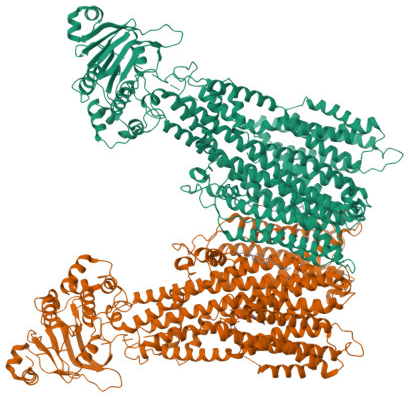
\includegraphics[width=2.3cm, height=2.3cm, keepaspectratio]{Figures/mrp1_estructura_cropped.png}
};

% --- Fila 3 (y = -1.1): Optimización y Decisión ---

% 8. Optimización Multiobjetivo (Columna 3: centro en x = 7.1, y = -1.1)
\node[
    draw=figGreen,
    fill=figGreenTint,
    rounded corners=5pt,
    line width=1.2pt,
    minimum width=3.2cm,
    minimum height=1.8cm,
    align=center,
    text=darkText
] (nodeMeta) at (7.1, -1.1) {
    {\fontsize{10.5}{13.5}\selectfont\textbf{\color{figGreen!80!black} Optimización}}\\[2pt]
    {\fontsize{10.5}{13.5}\selectfont\textbf{\color{figGreen!80!black} multiobjetivo}}
};

% 9. Decisión ¿Condición de parada? (Columna 5: centro en x = 13.2, y = -1.1)
\node[
    diamond,
    aspect=1.4,
    draw=darkText!80,
    fill=cardBorder!30,
    line width=1.1pt,
    inner sep=3pt,
    align=center,
    text=darkText
] (nodeCond) at (13.2, -1.1) {
    {\fontsize{9}{11}\selectfont\textbf{¿Condición}}\\[-1pt]
    {\fontsize{9}{11}\selectfont\textbf{de parada?}}
};

% --- Fila 4 (y = -3.4): Salida final ---

% 10. Mejores Moléculas (Columna 5: centro en x = 13.2, y = -3.4)
\node[
    draw=figVermilion!90!black,
    fill=figVermilionTint,
    rounded corners=5pt,
    line width=1.3pt,
    minimum width=2.6cm,
    minimum height=1.8cm,
    align=center,
    text=darkText
] (nodeMejores) at (13.2, -3.4) {
    {\fontsize{11}{14}\selectfont\textbf{\color{figVermilion!90!black} Mejores}}\\[2pt]
    {\fontsize{11}{14}\selectfont\textbf{\color{figVermilion!90!black} moléculas}}\\[3pt]
    {\scriptsize\color{grayText} Candidatas finales}
};

% =========================================================================
% 2. CONEXIONES
% =========================================================================

% VAE: MOSES -> Codificador (horizontal: longitud 0.7cm)
\draw[line width=1.1pt, draw=grayText!80, -{Stealth[length=5pt, width=3.5pt]}]
    (nodeMoses.east) -- (2.8, 4.8);

% VAE: Codificador -> Espacio Latente (horizontal: longitud 0.7cm)
\draw[line width=1.1pt, draw=grayText!80, -{Stealth[length=5pt, width=3.5pt]}]
    (5.6, 4.8) -- (nodeLatent.west);

% VAE: Espacio Latente -> Decodificador (horizontal: longitud 0.7cm)
\draw[line width=1.1pt, draw=grayText!80, -{Stealth[length=5pt, width=3.5pt]}]
    (nodeLatent.east) -- (8.6, 4.8);

% VAE: Decodificador -> Moléculas generadas (horizontal: longitud 0.7cm)
\draw[line width=1.1pt, draw=grayText!80, -{Stealth[length=5pt, width=3.5pt]}]
    (11.4, 4.8) -- (nodeMols.west);

% Evaluación: Moléculas generadas -> Calcular Aptitud (vertical hacia abajo: longitud 1.1cm)
\draw[line width=1.1pt, draw=grayText!80, -{Stealth[length=5pt, width=3.5pt]}]
    (nodeMols.south) -- (nodeAptitud.north);

% Evaluación: Proteína MRP1 -> Calcular Aptitud (horizontal hacia la izquierda: longitud 0.7cm)
\draw[line width=1.1pt, draw=grayText!80, -{Stealth[length=5pt, width=3.5pt]}]
    (imgMRP1.west) -- (nodeAptitud.east);

% Evaluación -> Decisión: Calcular Aptitud -> ¿Condición de parada? (vertical hacia abajo: longitud 0.85cm)
\draw[line width=1.1pt, draw=grayText!80, -{Stealth[length=5pt, width=3.5pt]}]
    (nodeAptitud.south) -- (nodeCond.north);

% Decisión: Rama SÍ -> Mejores Moléculas (vertical hacia abajo con holgura limpia)
\draw[line width=1.1pt, draw=darkText, -{Stealth[length=5pt, width=3.5pt]}]
    (nodeCond.south) -- (nodeMejores.north)
    node[pos=0.32, right=5pt, font=\footnotesize\bfseries, text=darkText] {SÍ};

% Decisión: Rama NO -> Optimización multiobjetivo (horizontal hacia la izquierda: longitud 3.1cm)
\draw[line width=1.1pt, draw=darkText, -{Stealth[length=5pt, width=3.5pt]}]
    (nodeCond.west) -- (nodeMeta.east)
    node[midway, above=3pt, font=\footnotesize\bfseries, text=darkText] {NO};

% Ciclo de Optimización: Optimización multiobjetivo -> Espacio Latente (vertical hacia arriba: longitud 3.2cm)
\draw[line width=1.2pt, draw=figGreen!80!black, -{Stealth[length=5pt, width=3.5pt]}]
    (nodeMeta.north) -- (nodeLatent.south);

\end{tikzpicture}%
}
\caption{Visión general de la metodología: arquitectura del VAE preentrenado con MOSES y ciclo iterativo de optimización multiobjetivo en el espacio latente para la generación de moléculas candidatas contra MRP1.}
\label{fig:pipeline_metodologia}
\end{figure}
